%%%%%%%% ICML 2021 EXAMPLE LATEX SUBMISSION FILE %%%%%%%%%%%%%%%%%

\documentclass{article}
\usepackage{float}
\usepackage{microtype}
\bibliographystyle{icml2021}
\usepackage{graphicx}
\usepackage{subfigure}
\usepackage{booktabs}
\usepackage{float}
\usepackage{gensymb}
\usepackage{amsmath}
\usepackage{amssymb}
\usepackage{tikz}

\usepackage{url}
\def\UrlBreaks{\do\/\do-}
\usepackage{breakurl}
\usepackage[breaklinks]{hyperref}
\usepackage{hyperref}

\newcommand{\theHalgorithm}{\arabic{algorithm}}
\newcommand{\TODO}[1]{\textcolor{blue}{#1}}

\usepackage[accepted]{icml2021}

\icmltitlerunning{Hyperparameter Tuning using Evolutionary Algorithms}

\begin{document}

\twocolumn[
\icmltitle{Hyperparameter Tuning using Evolutionary Algorithms}
\icmlsetsymbol{equal}{*}
\begin{icmlauthorlist}
    \icmlauthor{T. Blom (sXXXXXXXX)}{LIACS}
    \icmlauthor{J. Hamelink (s2233827)}{LIACS}
    \icmlauthor{L. Peeters (s2011174)}{LIACS}
    \icmlauthor{S. Sharma (s3772241)}{LIACS}
\end{icmlauthorlist}
\icmlaffiliation{LIACS}{LIACS, Leiden University, Leiden, Netherlands}
\icmlcorrespondingauthor{Mike Preuss}{LIACS}
\icmlkeywords{Hyperparameter Tuning, Evolutionary Algorithms, Reinforcement Learning}

\vskip 0.3in
]

\printAffiliationsAndNotice{}

% -------------------------------------------------------------------
% -------------------------------------------------------------------
\section{Introduction}
\label{sec:intro}
Hyperparameter tuning is an active research topic in machine learning that can have a significant impact on the performance of models. 
The process of manually fine-tuning hyperparameters can be time-consuming. 
In this study, we propose the use of a genetic algorithm as a means to optimize the hyperparameters of an Advantage Actor-Critic (A2C) agent. 
This includes the hyperparameters of the neural network the agent uses such as the number of layers, the number of neurons per layer, the activation functions employed, and the learning rate. Furthermore, hyperparameters of the A2C agent such as the discount factor, Entropy Regularization, and baseline subtraction. 
We aim to automate the exploration of various hyperparameter settings using a genetic algorithm, with the goal of finding an optimal combination. 
We use a bitstring representation to encode and manipulate the hyperparameter configuration. 
Each bit or set of bits within the string corresponds to a specific hyperparameter setting, allowing for easy manipulation by the genetic algorithm's evolutionary process. 
Similar to the process of natural selection and genetics, the genetic algorithm starts with an initial population of bitstrings and iteratively tries to improve them with the goal of finding an optimal configuration of hyperparameters. 
To evaluate the performance and effectiveness of our Hyperparameter Optimization (HPO) algorithm for the A2C agent, we apply the agent on three of OpenAI's Gym environments: CartPole-v1, Acrobot-v1, and LunarLander-v2. 
These environments provide varying sizes of action and observation spaces, enabling a more generalized assessment of the HPO algorithm's performance.
In this study, we aim to investigate the impact of our genetic algorithm-based HPO approach on the performance and convergence speed of the A2C agent in various Gym environments. 

% -------------------------------------------------------------------
% -------------------------------------------------------------------
\section{Methodology}
\label{sec:meth}

\TODO{small intro for this section.}

% -------------------------------------------------------------------
\subsection{Advantage Actor-Critic (A2C) Algorithm}
\label{ssec:A2C}

The Advantage Actor-Critic (A2C) algorithm is a policy gradient-based reinforcement learning method.
It uses a two-headed neural network to simultaneously estimate the policy (actor) and value function (critic) to improve the agent's performance.
In this section, we describe the A2C algorithm and which corresponding hyperparameters we intend to tune using a Genetic Algorithm (GA).


% -------------------------------------------------------------------
\subsubsection{Two-Headed Neural Network}
\label{sssec:2hnn}

The Advantage Actor-Critic (A2C) and Actor-Critic (AC) algorithms both use a two-headed neural network architecture, consisting of an actor head and a critic head.
However, in AC algorithms, the actor and critic are updated asynchronously.
While A2C introduces synchronous updates of the two heads, with the goal of mitigating potential instabilities associated with asynchronous updates.
In A2C, the two heads are updated simultaneously using a single neural network.
The actor head provides the action probabilities, and the critic head estimates the state-value function.
The training of both heads is performed using the advantage function, which calculates the advantage of taking a specific action compared to the average action value in the state.

\begin{algorithm}[H]
    \caption{A2C Algorithm with Baseline Subtraction and Entropy Regularization}
  \label{alg:A2C}
  \begin{algorithmic}[1]
      \REQUIRE Number of episodes $N$, learning rate $\alpha$, discount factor $\gamma$
      \STATE Initialize Actor $\pi(s, a; \theta)$ and Critic $V(s; \omega)$ network.
      \FOR{\textbf{Episode} $= 1$ to $N$}
          \STATE Initialize state $s$
    
          \WHILE{\textbf{Episode} not finished}
              \STATE Select action $a$ from the actor network with state $s$
              \STATE Execute action $a$ and observe next state $s'$ and reward $r$
      
              \STATE Calculate estimated value $V(s; \omega)$
              \STATE Calculate advantage $A = r + \gamma V(s'; \omega) - V(s; \omega)$
      
              \STATE Update the critic network by minimizing the mean squared error loss:
              \STATE $\quad \mathcal{L}_{\textbf{CRITIC}} = (r + \gamma V(s'; \omega) - V(s; \omega))^2$
      
              \STATE Update the actor network using the advantage as the policy gradient, with baseline subtraction:
              \STATE $\quad \mathcal{L}_{\textbf{ACTOR}} = -\log \pi(a|s; \theta) \cdot (A - V(s; \omega))$
      
              \STATE Calculate the entropy of the actor's distribution:
              \STATE $\quad \text{Entropy} = -\sum_{a} \pi(a|s; \theta) \log \pi(a|s; \theta)$
      
              \STATE Update both networks using gradient descent
      
              \STATE Update state $s$ to $s'$
      \ENDWHILE
      \ENDFOR
    \end{algorithmic}
\end{algorithm}

% -------------------------------------------------------------------
\subsubsection{Entropy Regularization}
\label{sssec:entreg}

The agent's policy is a probability distribution over all possible actions in the current state.
Higher entropy in this distribution causes more randomness in the action selection.
Using entropy regularization in the A2C algorithm thus encourages exploration to prevent the agent from getting stuck in suboptimal solutions.
In the objective function of A2C below we can see that the amount of entropy regularization is controlled by hyperparameter $\beta$.
By tuning this $\beta$ we can influence the agent's balance between exploration and exploitation and optimize its performance.

\[
\mathcal{J}(\theta) = \sum_{t} \left( \log(\pi(a_t|s_t)) \cdot A(s_t, a_t) - \beta \cdot \mathcal{H}(\pi(s_t)) \right)
\]
The objective function consists of three parts: the log probability of the selected action $\log(\pi(a_t|s_t))$, the advantage function $A(s_t, a_t)$, and the entropy regularization term $\mathcal{H}(\pi(s_t))$weighted by hyperparameter $\beta$

\subsubsection{Baseline Subtraction}
\label{sssec:blsub}

Baseline subtraction is a technique used to reduce the variance of the policy gradient estimates during training.
It involves subtracting a baseline value from the estimated returns or advantages before updating the policy.
For our HPO algorithm, we will have encoded baseline subtraction with a single bit, 1 means the A2C agent will use baseline subtraction, and 0 means no baseline subtraction.

\subsubsection{Advantage Estimation (Calculating Returns)}
\label{sssec:advest}

The A2C algorithm utilizes advantage estimation to approximate the advantage function.
This function gives the advantage of taking a specific action in a given state compared to the average value of actions in that state.
The advantage is calculated by subtracting the estimated state-value function (critic's output) from the observed returns obtained during the interaction with the environment.
The returns are computed as the sum of discounted future rewards. 
The discount factor is another hyperparameter we will try to optimize, for it we will try four values: 0.9, 0.99, 0.995, and 0.999.


% -------------------------------------------------------------------
\subsection{Evolutionary Algorithm}
\label{ssec:EA}

The hyperparameter configuration for the Actor-Critic network will be optimized using an Evolutionary Algorithm (EA) \cite{Simon2013EvolutionaryOA}.
EA is a metaheuristic population-based algorithm that is inspired by biological evolution.
Pseudocode for EA is presented in Algorithm \ref{alg:EA}.

\begin{algorithm}[htbp]
    \caption{Evolutionary Algorithm}
    \label{alg:EA}
    \begin{algorithmic}[1]
        \STATE population $\gets$ random values
        \STATE candidate $\gets$ None
        \STATE max$\_$fitness $\gets$ -$\infty$
        
        \FOR {$N_{generations}$}
            \STATE fitness $\gets$ evaluate population
            \IF {max(fitness) $>$ max$\_$fitness}
            	\STATE max$\_$fitness $\gets$ max(fitness)
            	\STATE candidate $\gets$ best individual
            \ENDIF
            \STATE Select $\mu$ candidates
            \STATE Generate offspring via crossover
            \STATE Mutate population
        \ENDFOR        
    \end{algorithmic}
\end{algorithm}


The initial population is generated randomly.
After the population is created, the individuals are evaluated, in this case by using the hyperparameters corresponding to the individual to train the actor-critic network and evaluating it as described in section \ref{ssec:A2C}.
The resulting performance is called the individual's fitness value. 

Using the fitness values we select a subset $\mu$ of the population to reproduce, similar to how only fit individuals in a population in nature are able to find a mate.
Selection is done greedily, which does not allow for any exploration of the search space and makes it is rather likely that the algorithm gets stuck in local minima.
The greedy approach was chosen because of limited training resources.
While the minimum found by a greedy approach might not be the best, it is found and explored quickly, allowing for a good proof of concept result.

The selected individuals reproduce via a process known as crossover.
Biologically, this refers to the crossing of chromosomes, leading to two new chromosomes that have part of the DNA of one parent, and part of the other.
The algorithmic implementation of this process is very similar; take two selected parents and choose a random index where crossover occurs.
One offspring gets the first part of parent 1 and the second part of parent 2, and another offspring gets the inverse.
As such, each pair of two parents also creates two offspring.
This process repeats until the set of offspring, named $\lambda$, is of the desired size. 

In nature each generation consists of only offspring.
Parents continue to age, no matter how fit they are, and eventually become infertile and die.
This is called a $(\mu, \lambda)$ process, where the parents are replaced by the offspring.
Computer scientists have the luxury that the individuals do not age, so fit parents can be kept as long as is needed.
This allows for a $(\mu+\lambda)$ algorithm, which is the form used in this paper.
By allowing individuals to survive as long as they are fit enough, the algorithm can converge on a solution quicker. However, similar to the selection process, this sacrifices the ability to explore the search space. 

After creating offspring using crossover, the final step is mutation.
In nature, genes can randomly be mutated through accidents during the replicating process or exposure to radiation.
Generally, this is the main source of variation in biological populations.
This project makes use of uniform mutation, where each bit of each individual has a small chance of being flipped.
Mutation is the final step in creating a new generation, which can now be evaluated and go through the full process again.

% EXAMPLE TABLE
\begin{table}[htbp]
    \centering
    \begin{tabular}
        {|c|c|}
        \toprule
        \textbf{Parameter} & \textbf{Value} \\
        \midrule
        population size & 6 \\
        $\mu$           & 3 \\
        $\lambda$       & 3 \\
        mutation rate   & 0.1 \\
        \bottomrule
    \end{tabular}
    \caption{Hyperparameters}
    \label{tab:hyper}
\end{table}

% -------------------------------------------------------------------
% -------------------------------------------------------------------
\section{Experiments}
\label{sec:exp}

In order to test the effectiveness of the hyperparameter optimization algorithm, we will use it to optimize the hyperparameters of the A2C algorithm for three different environments: CartPole, Acrobot, and LunarLander.
In Cartpole, the algorithm is presented with a cart on a frictionless track has to balance a pole atop itself. 
A state consists of four continuous variables: Cart position, cart velocity, pole angle and pole angular velocity. 
The action space consists of a single discrete variable that represents a constant force being applied to the left or right of the cart, or not at all. 
Acrobot is a similar environment, where two linked poles hang from a fixed points. 
By applying force onto the link between the poles, the agent has to swing the free end of the chain above a height treshold. 
The action space consists of a single discrete variable that represents a constant force being applied to the chain. 
The state space contains six continuous variables: the sine, cosine and angular velocity of the two angles that define the orientation of the chain. 
Lunar Lander is an environment where a moonlander is descending to the moon, and the agent has to control engines to allow it to land safely. 
The action space is a discrete variable the represents firing one of the three engines, or doing nothing. 
The state space contains six continuous and two discrete variables: The coordinates of the lander, its linear velocities, its angle, its angular velocity, and two booleans that represent whether each leg is in contact with the ground or not.

Each of these environments is relatively simple for the agent to solve, allowing for the experiments to reach results over limited training resources. 
In addition, they all have discrete action spaces and relatively simple state spaces that do not require convolutional layers.

In total, eleven hyperparameters will be optimized as shown in Table \ref{tab:optimized_parameters}. 
The Evolutionary Algorithm is designed to optimize a bitstring, therefore each hyperparameter was assigned a discrete search space of either two or four possible option. 
This makes it easy to decode the bitstring into a hyperparameter configuration for the actor-critic network. 

\begin{table}[htbp]
    \centering
    \begin{tabular}
        {|c|c|}
        \toprule
        \textbf{Parameter} & \textbf{Search Space} \\
        \midrule
        Discount factor & [0.9, 0.99, 0.995, 0.999] \\
        Entropy Regularization weight & [0.0001, 0.001, 0.01, 0.1] \\
        Baseline Subtraction & [True, False] \\
        \midrule
        Number of hidden layers & [1, 2, 3, 4] \\
        Dropout rate & [0.01, 0.1, 0.2, 0.3] \\
        Hidden layer size & [32, 64, 128, 256] \\
        Hidden layer activation & [ReLU, Sigmoid] \\
        \midrule
        Learning rate & [0.1, 0.05, 0.01, 0.005] \\
        Learning rate decay & [1, 0.99, 0.9, 0.85] \\
        Learning rate step & [50, 100, 500, 1000] \\
        \bottomrule
    \end{tabular}
    \caption{Hyperparameters to be optimized by the Evolutionary Algorithm and their discrete search space. }
    \label{tab:optimized_parameters}
\end{table}

\TODO{Replace the default values by the ones we actually used}
For each environment, the Evolutionary Algorithm was given a population size of four individuals and was optimized for five generations. 
Each hyperparameter configuration was trained three seperate times. Every instance was trained for 1000 episodes and evaluated for 100 episodes.
The mean reward of the three configurations was then used as the evaluation metric and fitness function.   

% -------------------------------------------------------------------
% -------------------------------------------------------------------
\section{Results}
\label{sec:res}

\TODO{
    For each of the subsections, small introduction of what is to be expected.
    Then graphs and tables.
    Then (not super in-depth) analysis of the results.
}

% -------------------------------------------------------------------
\subsection{CartPole}
\label{ssec:cp}
\begin{figure}[htbp]
    \centering
    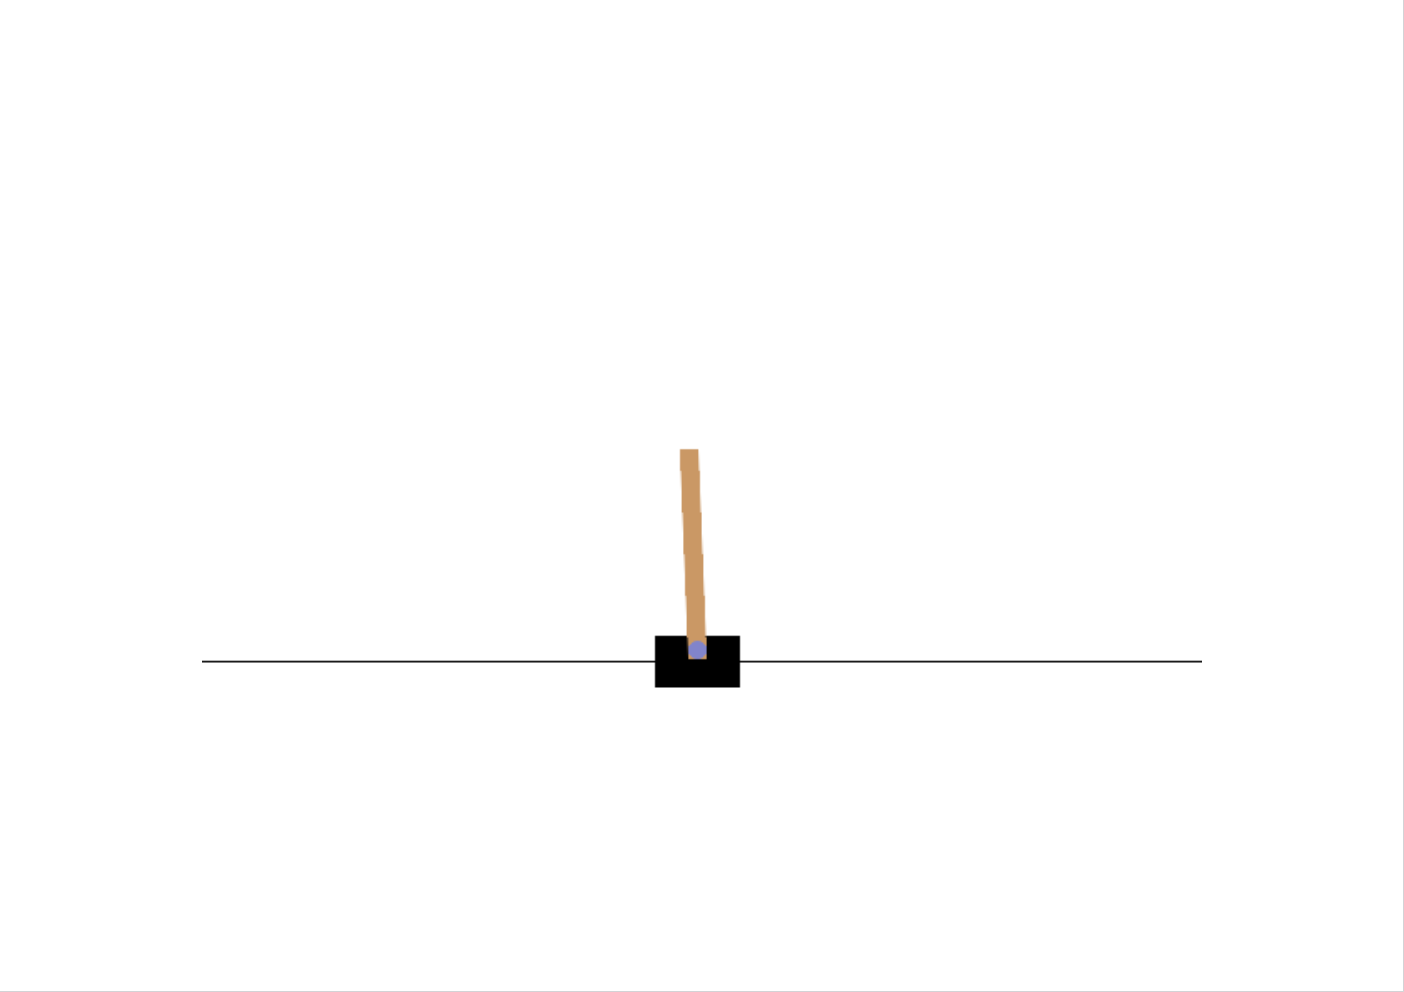
\includegraphics[width=0.9\linewidth]{figs/cartpole.png}
    \caption{
        OpenAI's CartPole environment. 
        Source: \cite{gymlibraryCartPole}
    }
    \label{fig:cartpole}
\end{figure}

\begin{figure}[htbp]
    \centering
    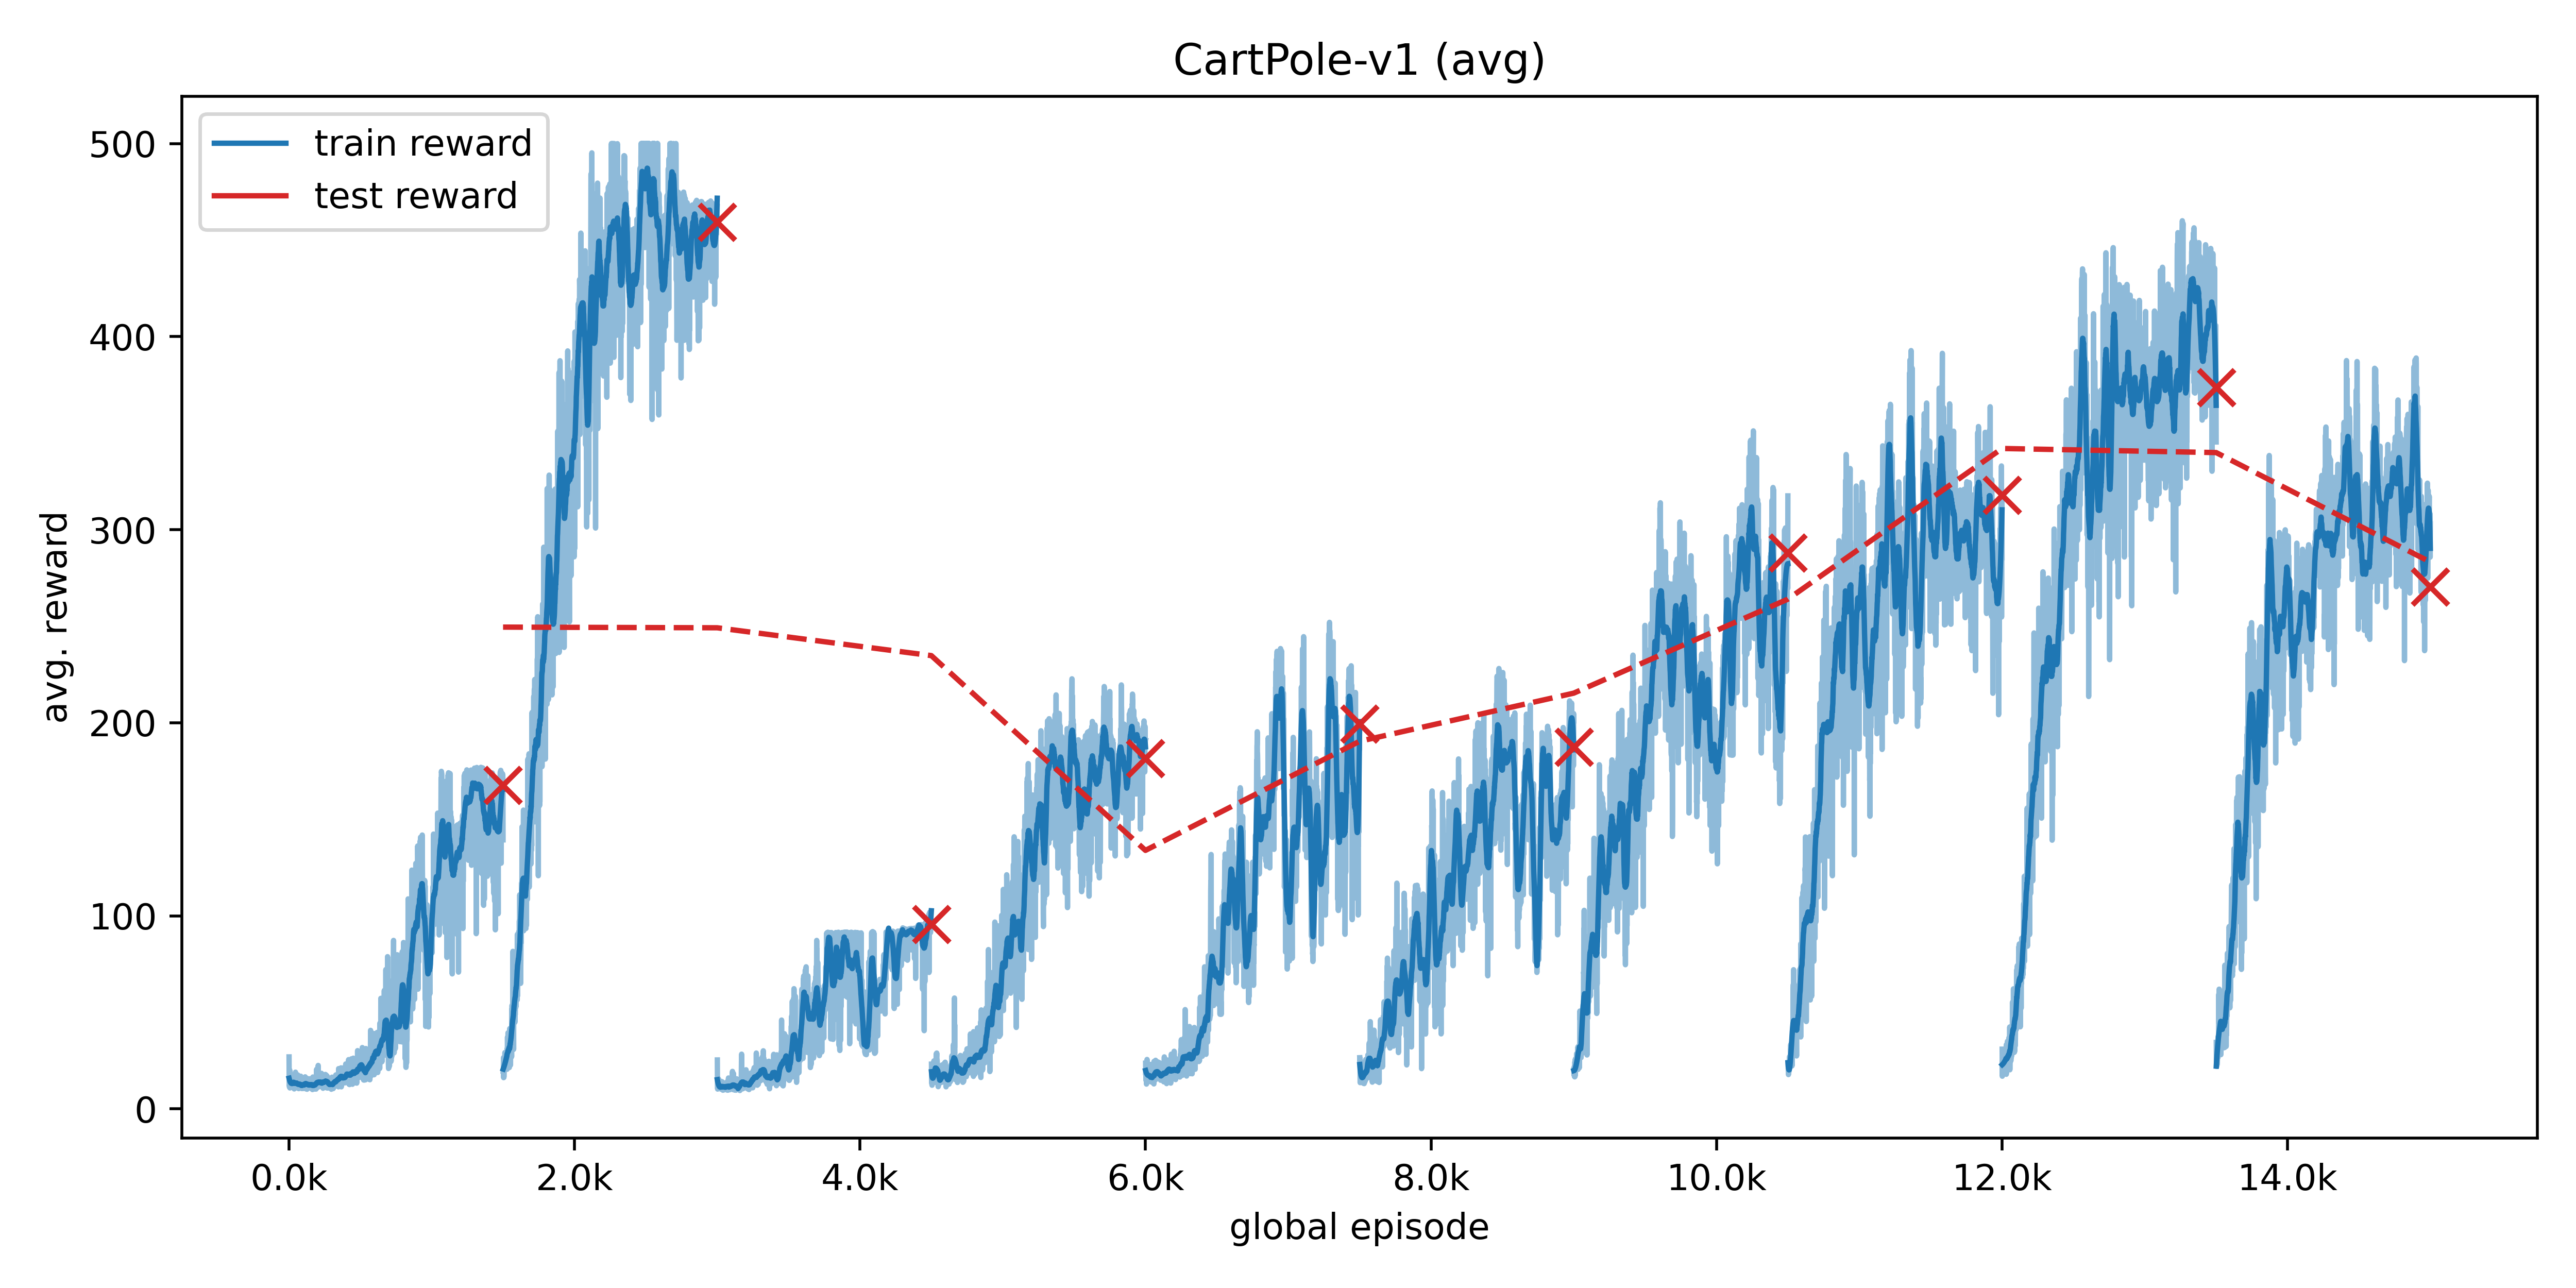
\includegraphics[width=0.9\linewidth]{figs/cp_avg_rewards.png}
    \caption{
        Average reward per global episode number for the CartPole environment.
    }
    \label{fig:avg-cp}
\end{figure}

\begin{figure}[htbp]
    \centering
    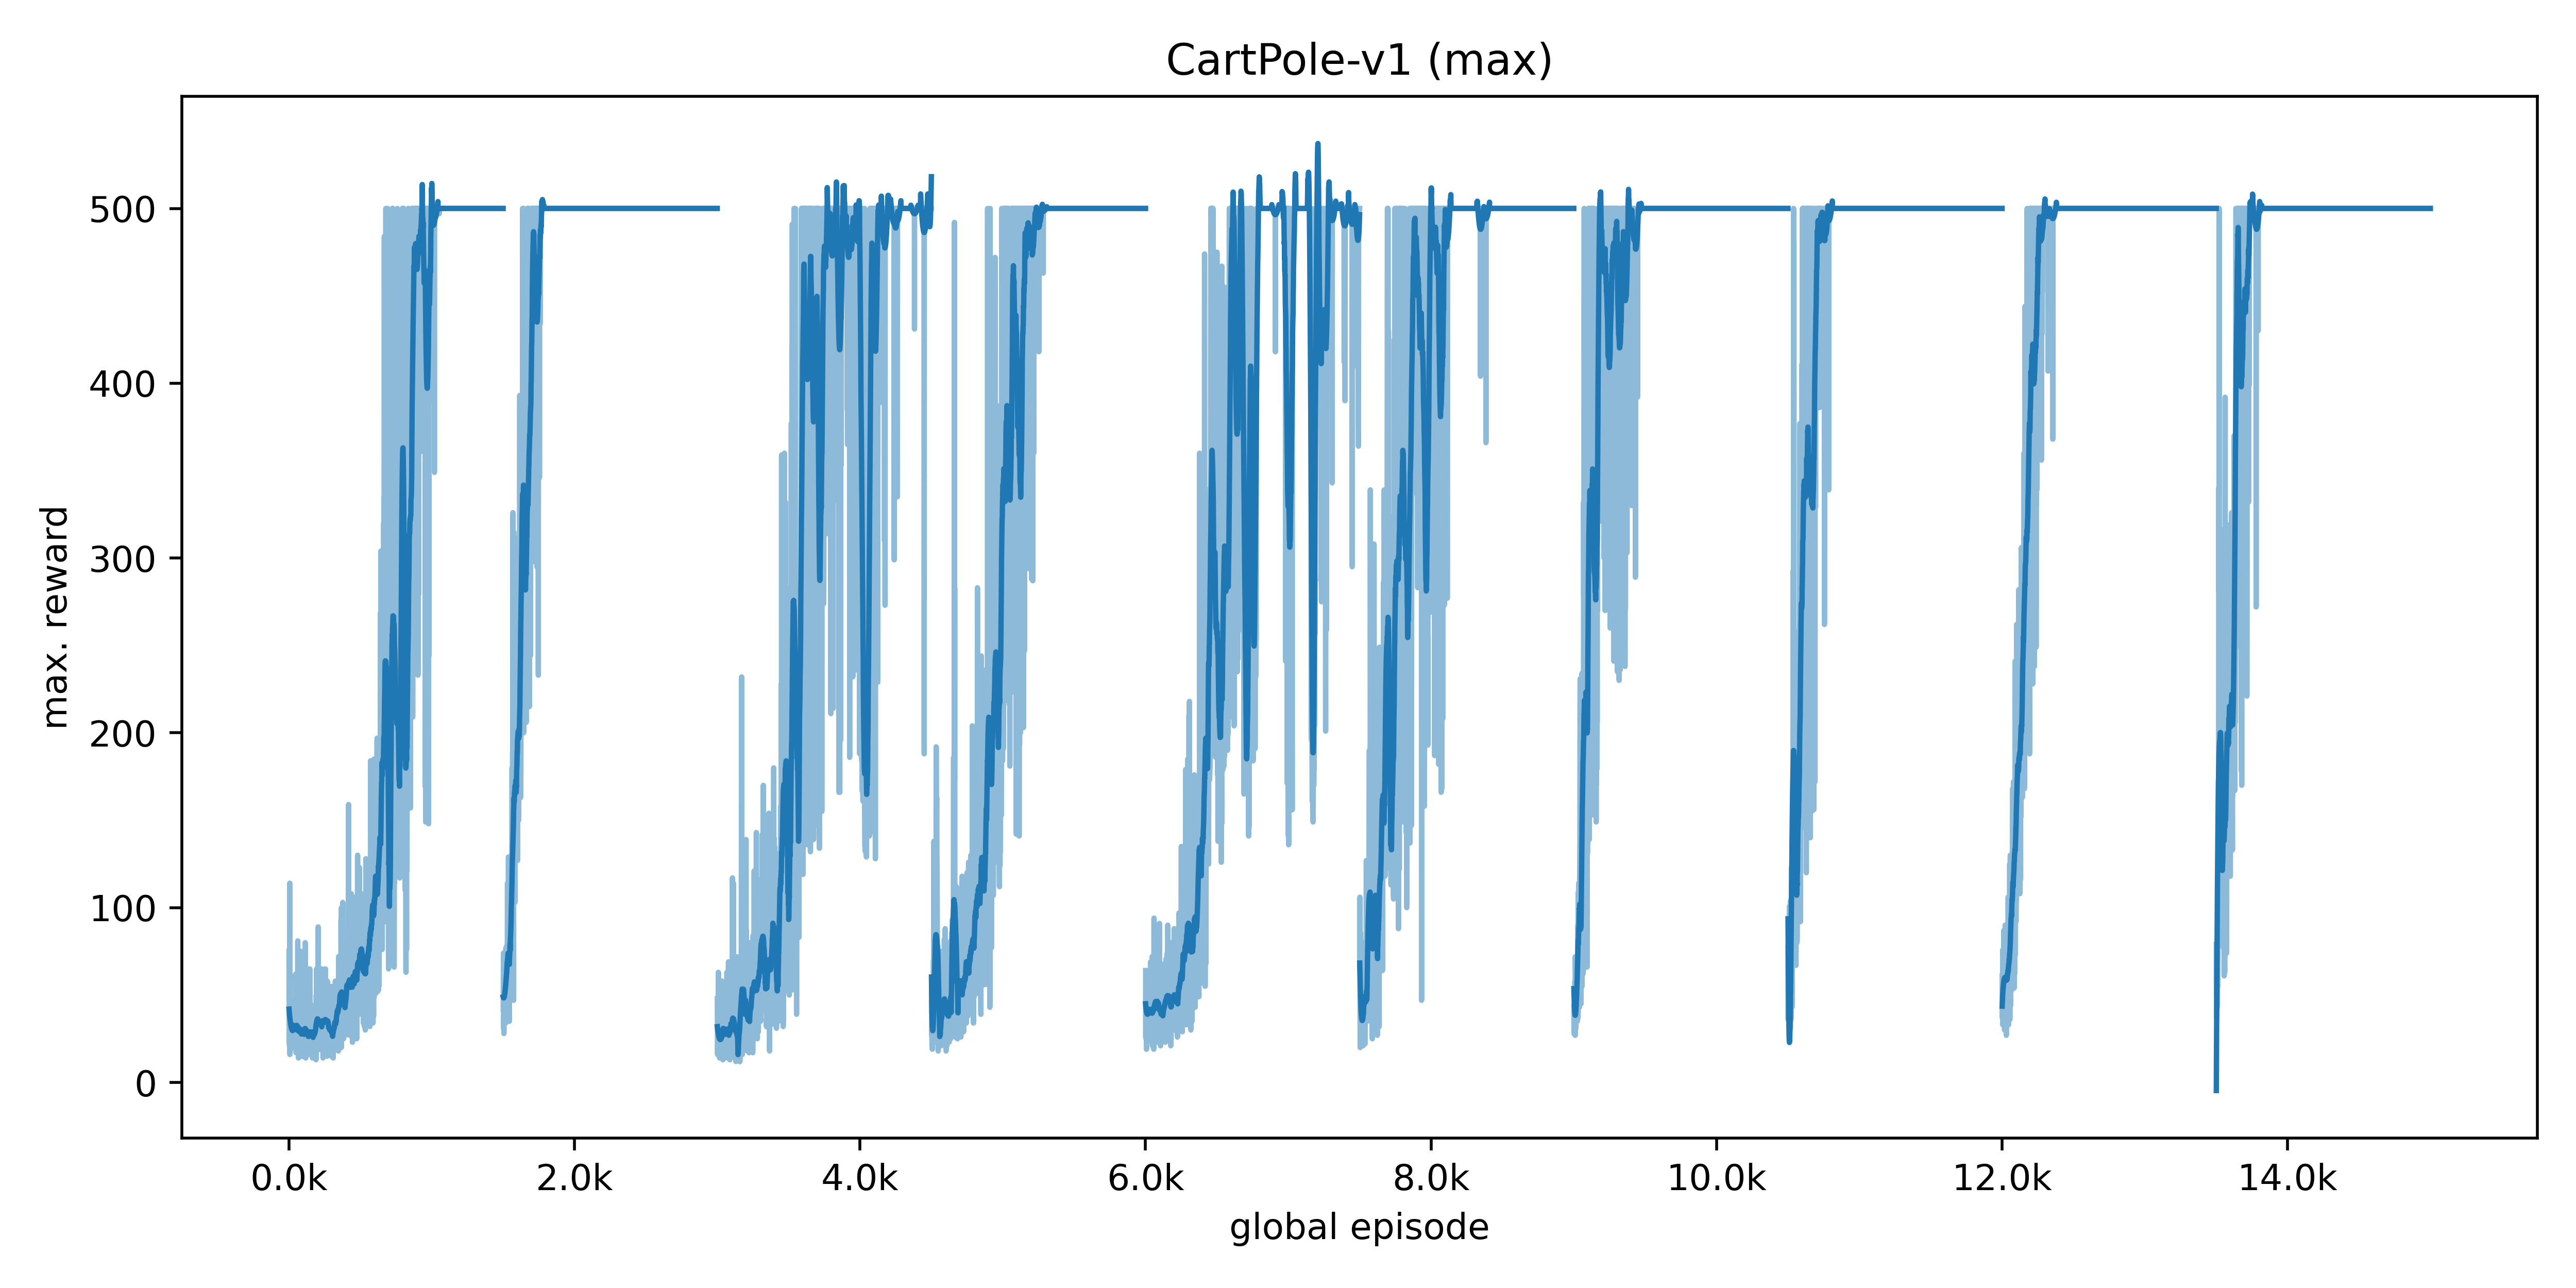
\includegraphics[width=0.9\linewidth]{figs/cp_max_rewards.png}
    \caption{
        Maximum reward per global episode number for the CartPole environment.
    }
    \label{fig:max-cp}
\end{figure}

% -------------------------------------------------------------------
\subsection{Acrobot}
\label{ssec:ab}

\begin{figure}[htbp]
    \centering
    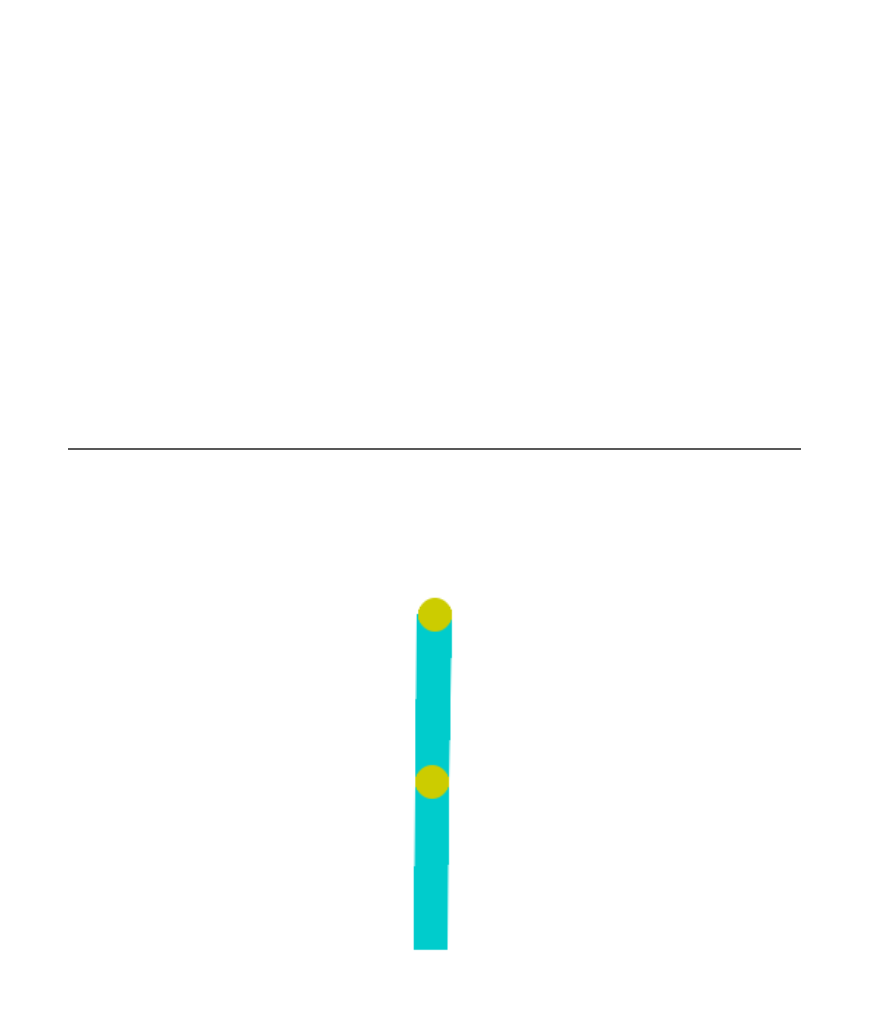
\includegraphics[width=0.9\linewidth]{figs/acrobot.png}
    \caption{
        OpenAI's CartPole environment. 
        Source: \cite{gymlibraryAcrobot}
    }
    \label{fig:acrobot}
\end{figure}

\begin{figure}[htbp]
    \centering
    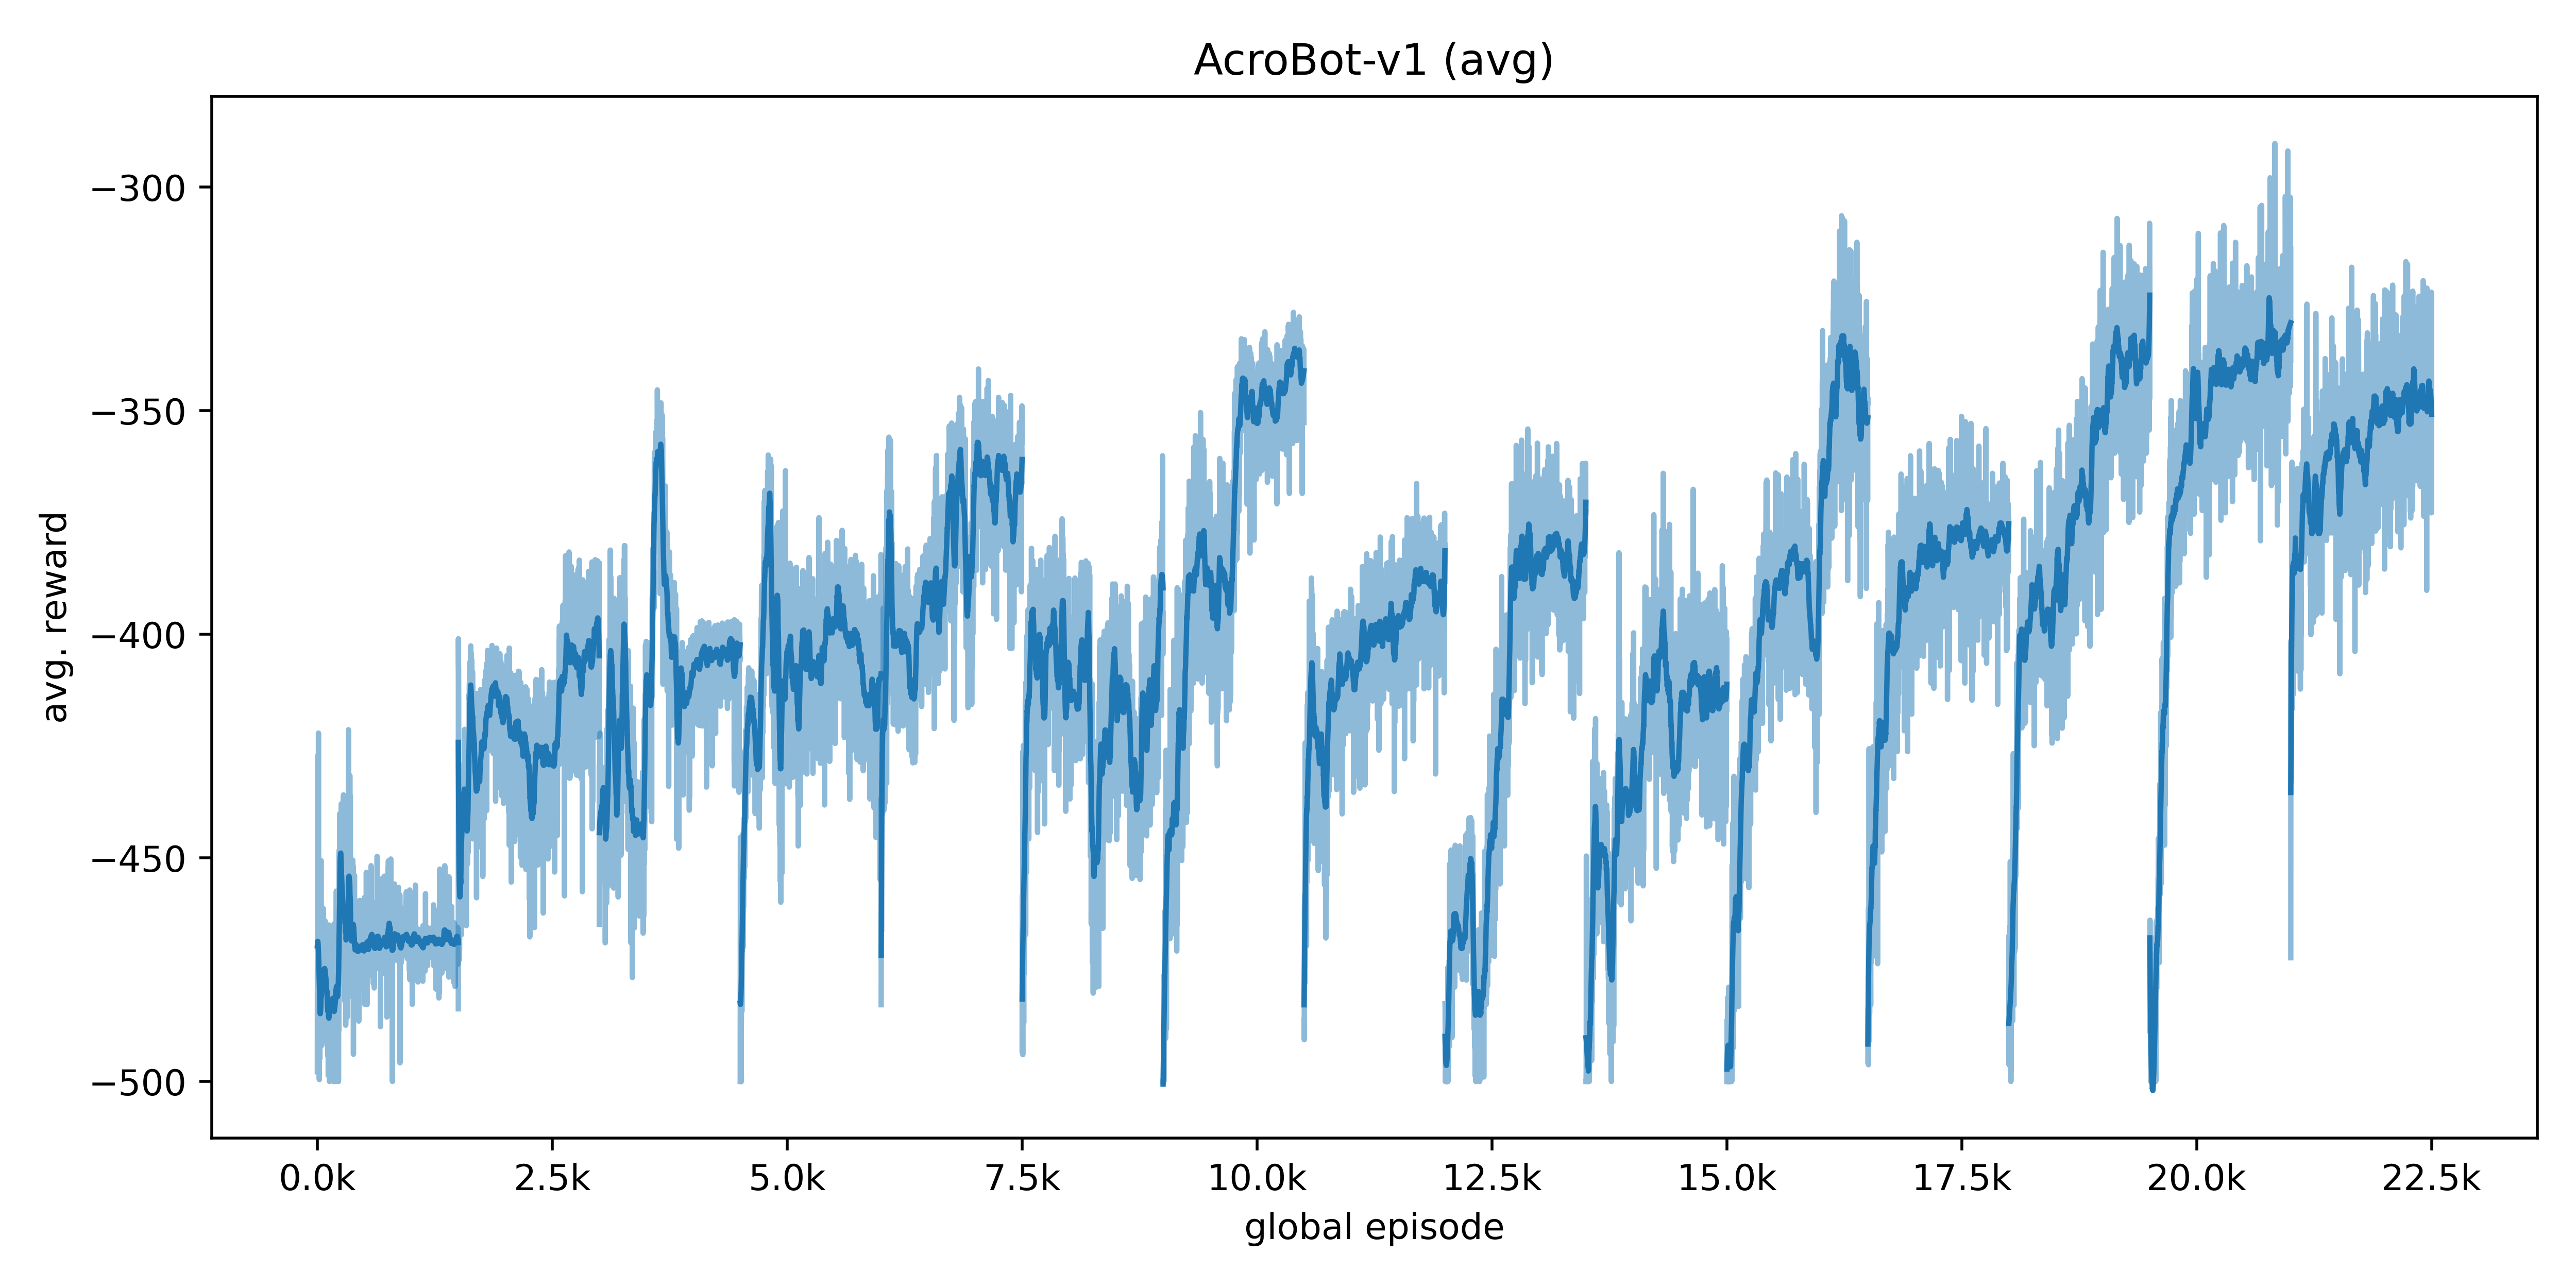
\includegraphics[width=0.9\linewidth]{figs/ab_avg_rewards.png}
    \caption{
        Average reward per global episode number for the AcroBot environment.
    }
    \label{fig:avg-ab}
\end{figure}

\begin{figure}[htbp]
    \centering
    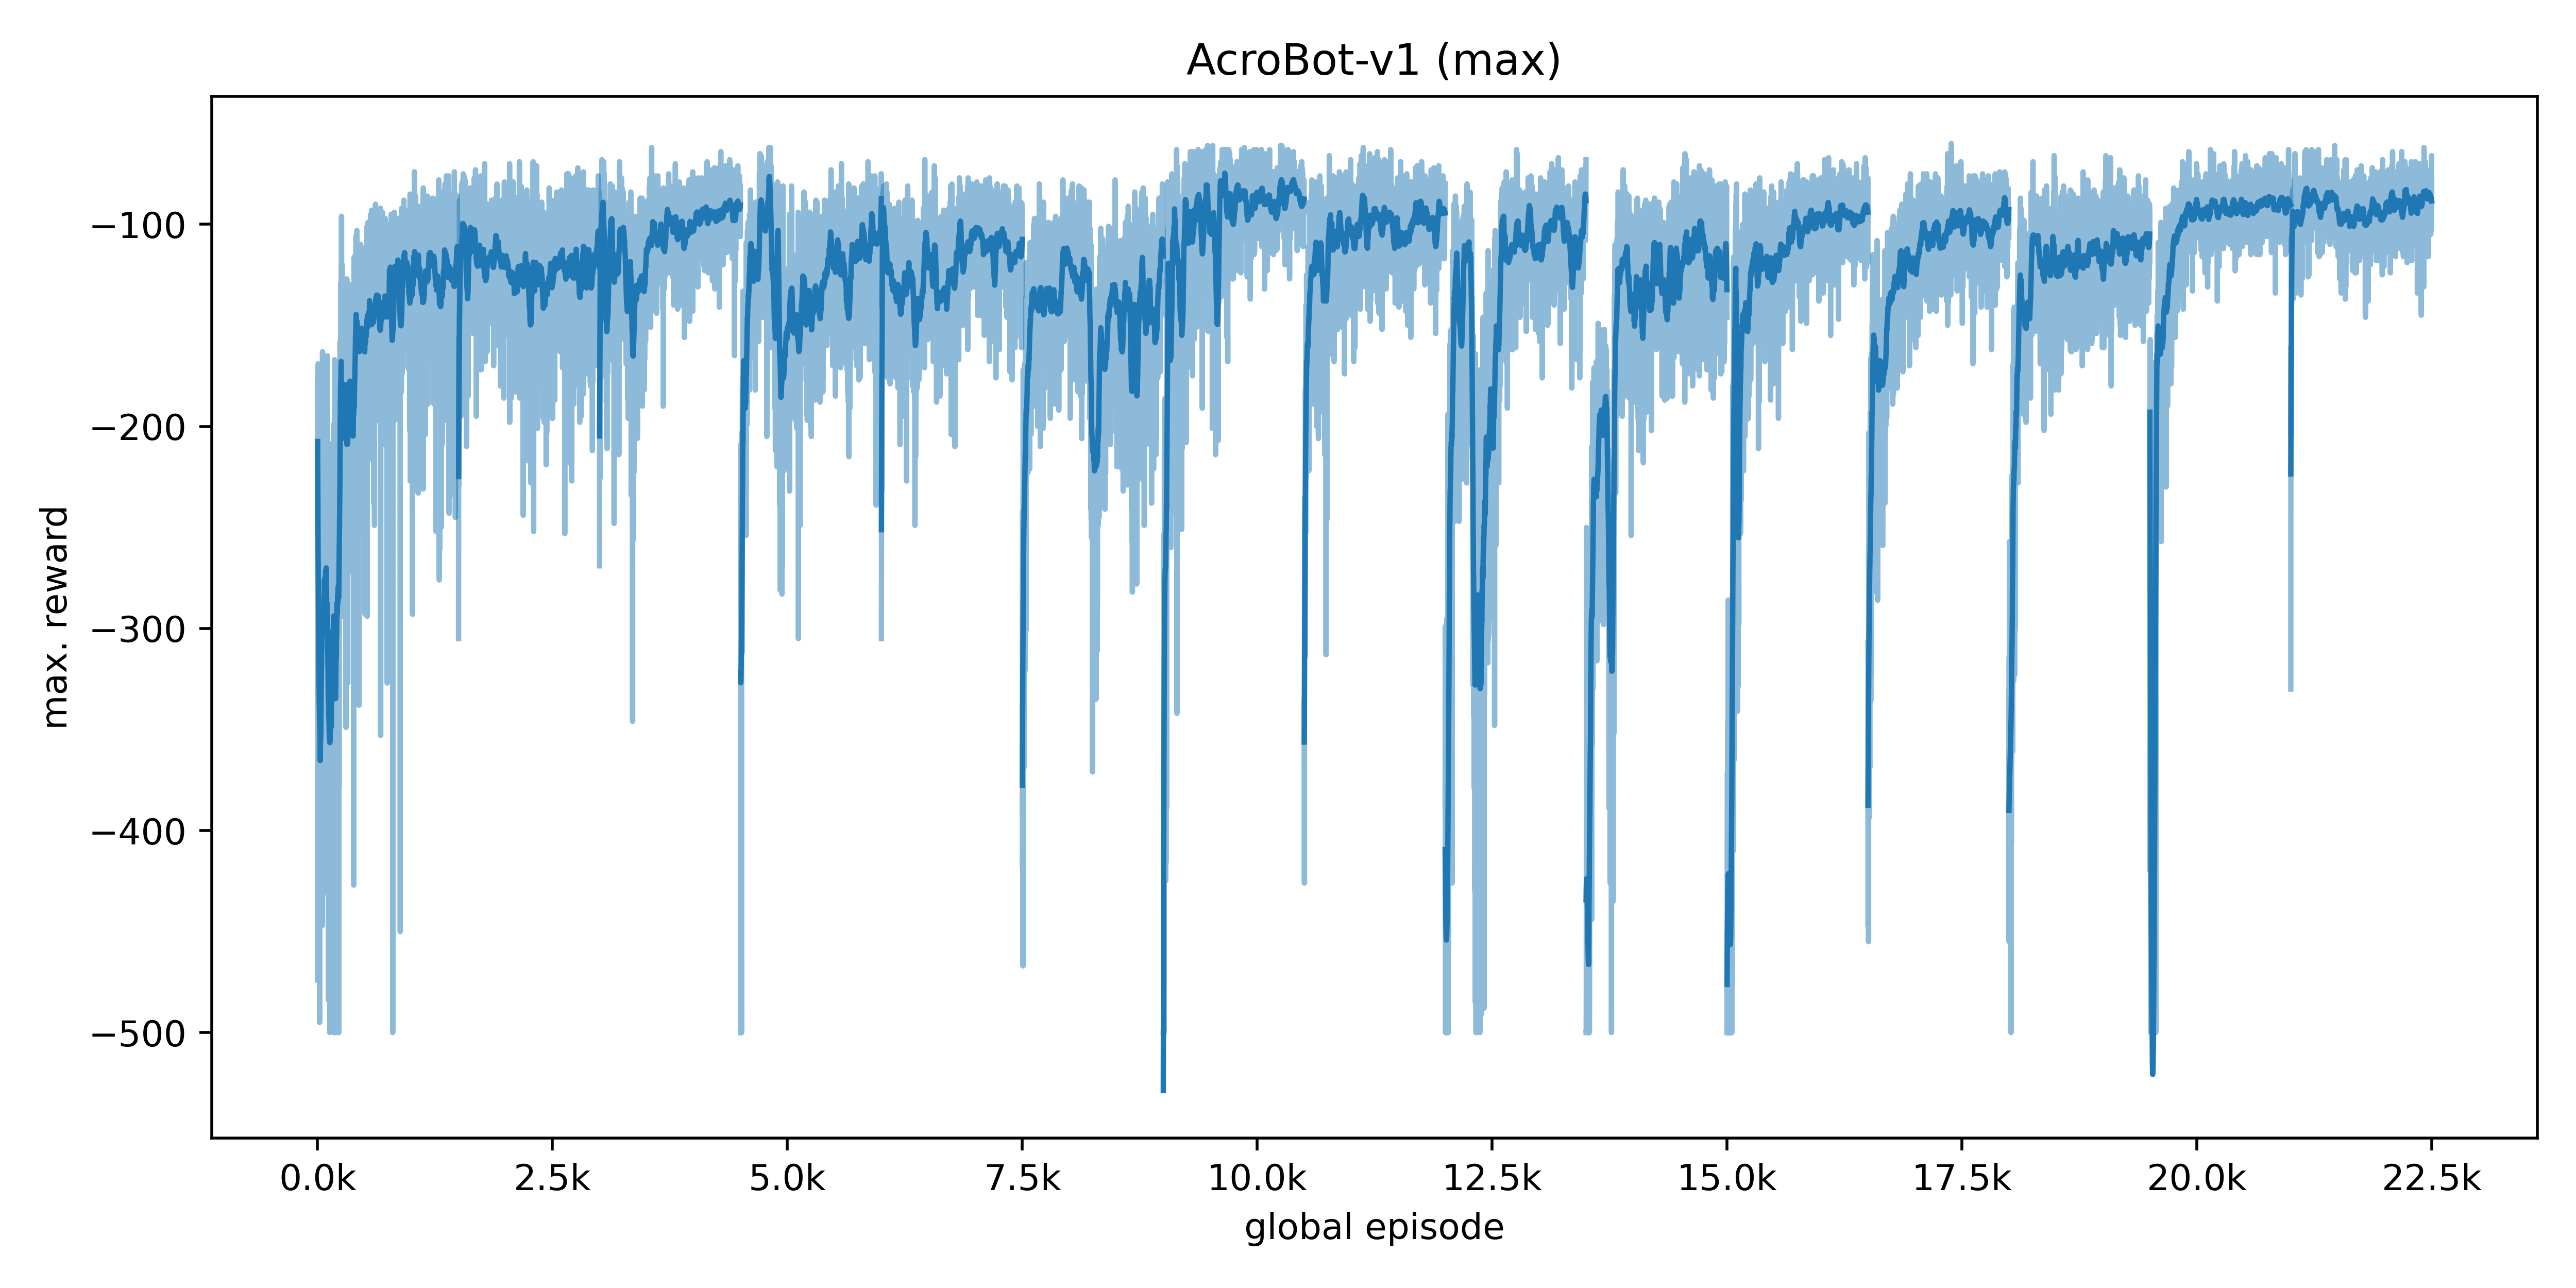
\includegraphics[width=0.9\linewidth]{figs/ab_max_rewards.png}
    \caption{
        Maximum reward per global episode number for the AcroBot environment.
    }
    \label{fig:max-ab}
\end{figure}

% -------------------------------------------------------------------
\subsection{LunarLander}
\label{ssec:ll}

\begin{figure}[htbp]
    \centering
    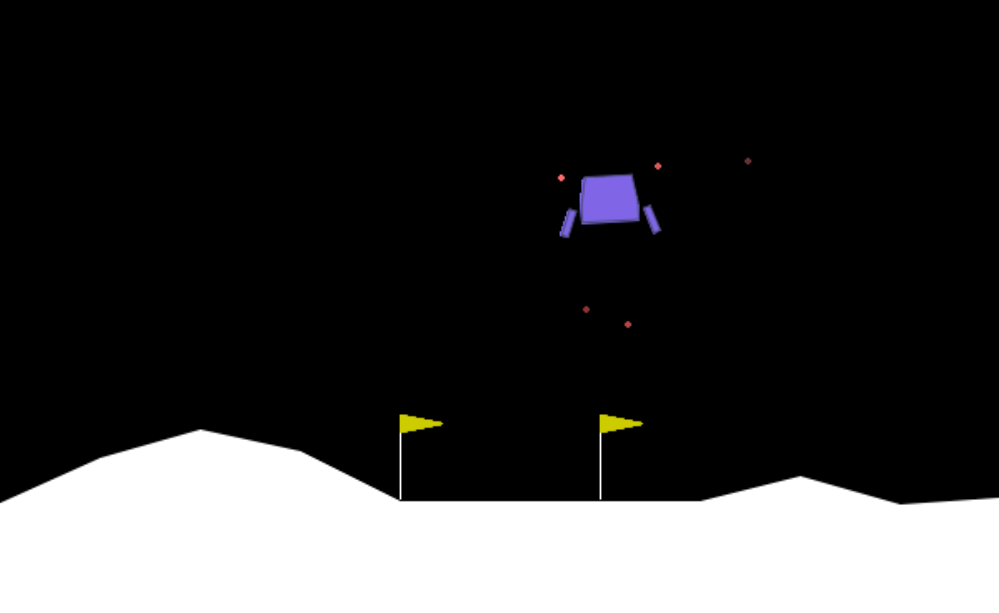
\includegraphics[width=0.9\linewidth]{figs/lunarlander.png}
    \caption{
        OpenAI's CartPole environment. 
        Source: \cite{gymlibraryLunarLander}
    }
    \label{fig:lunarlander}
\end{figure}

\begin{figure}[htbp]
    \centering
    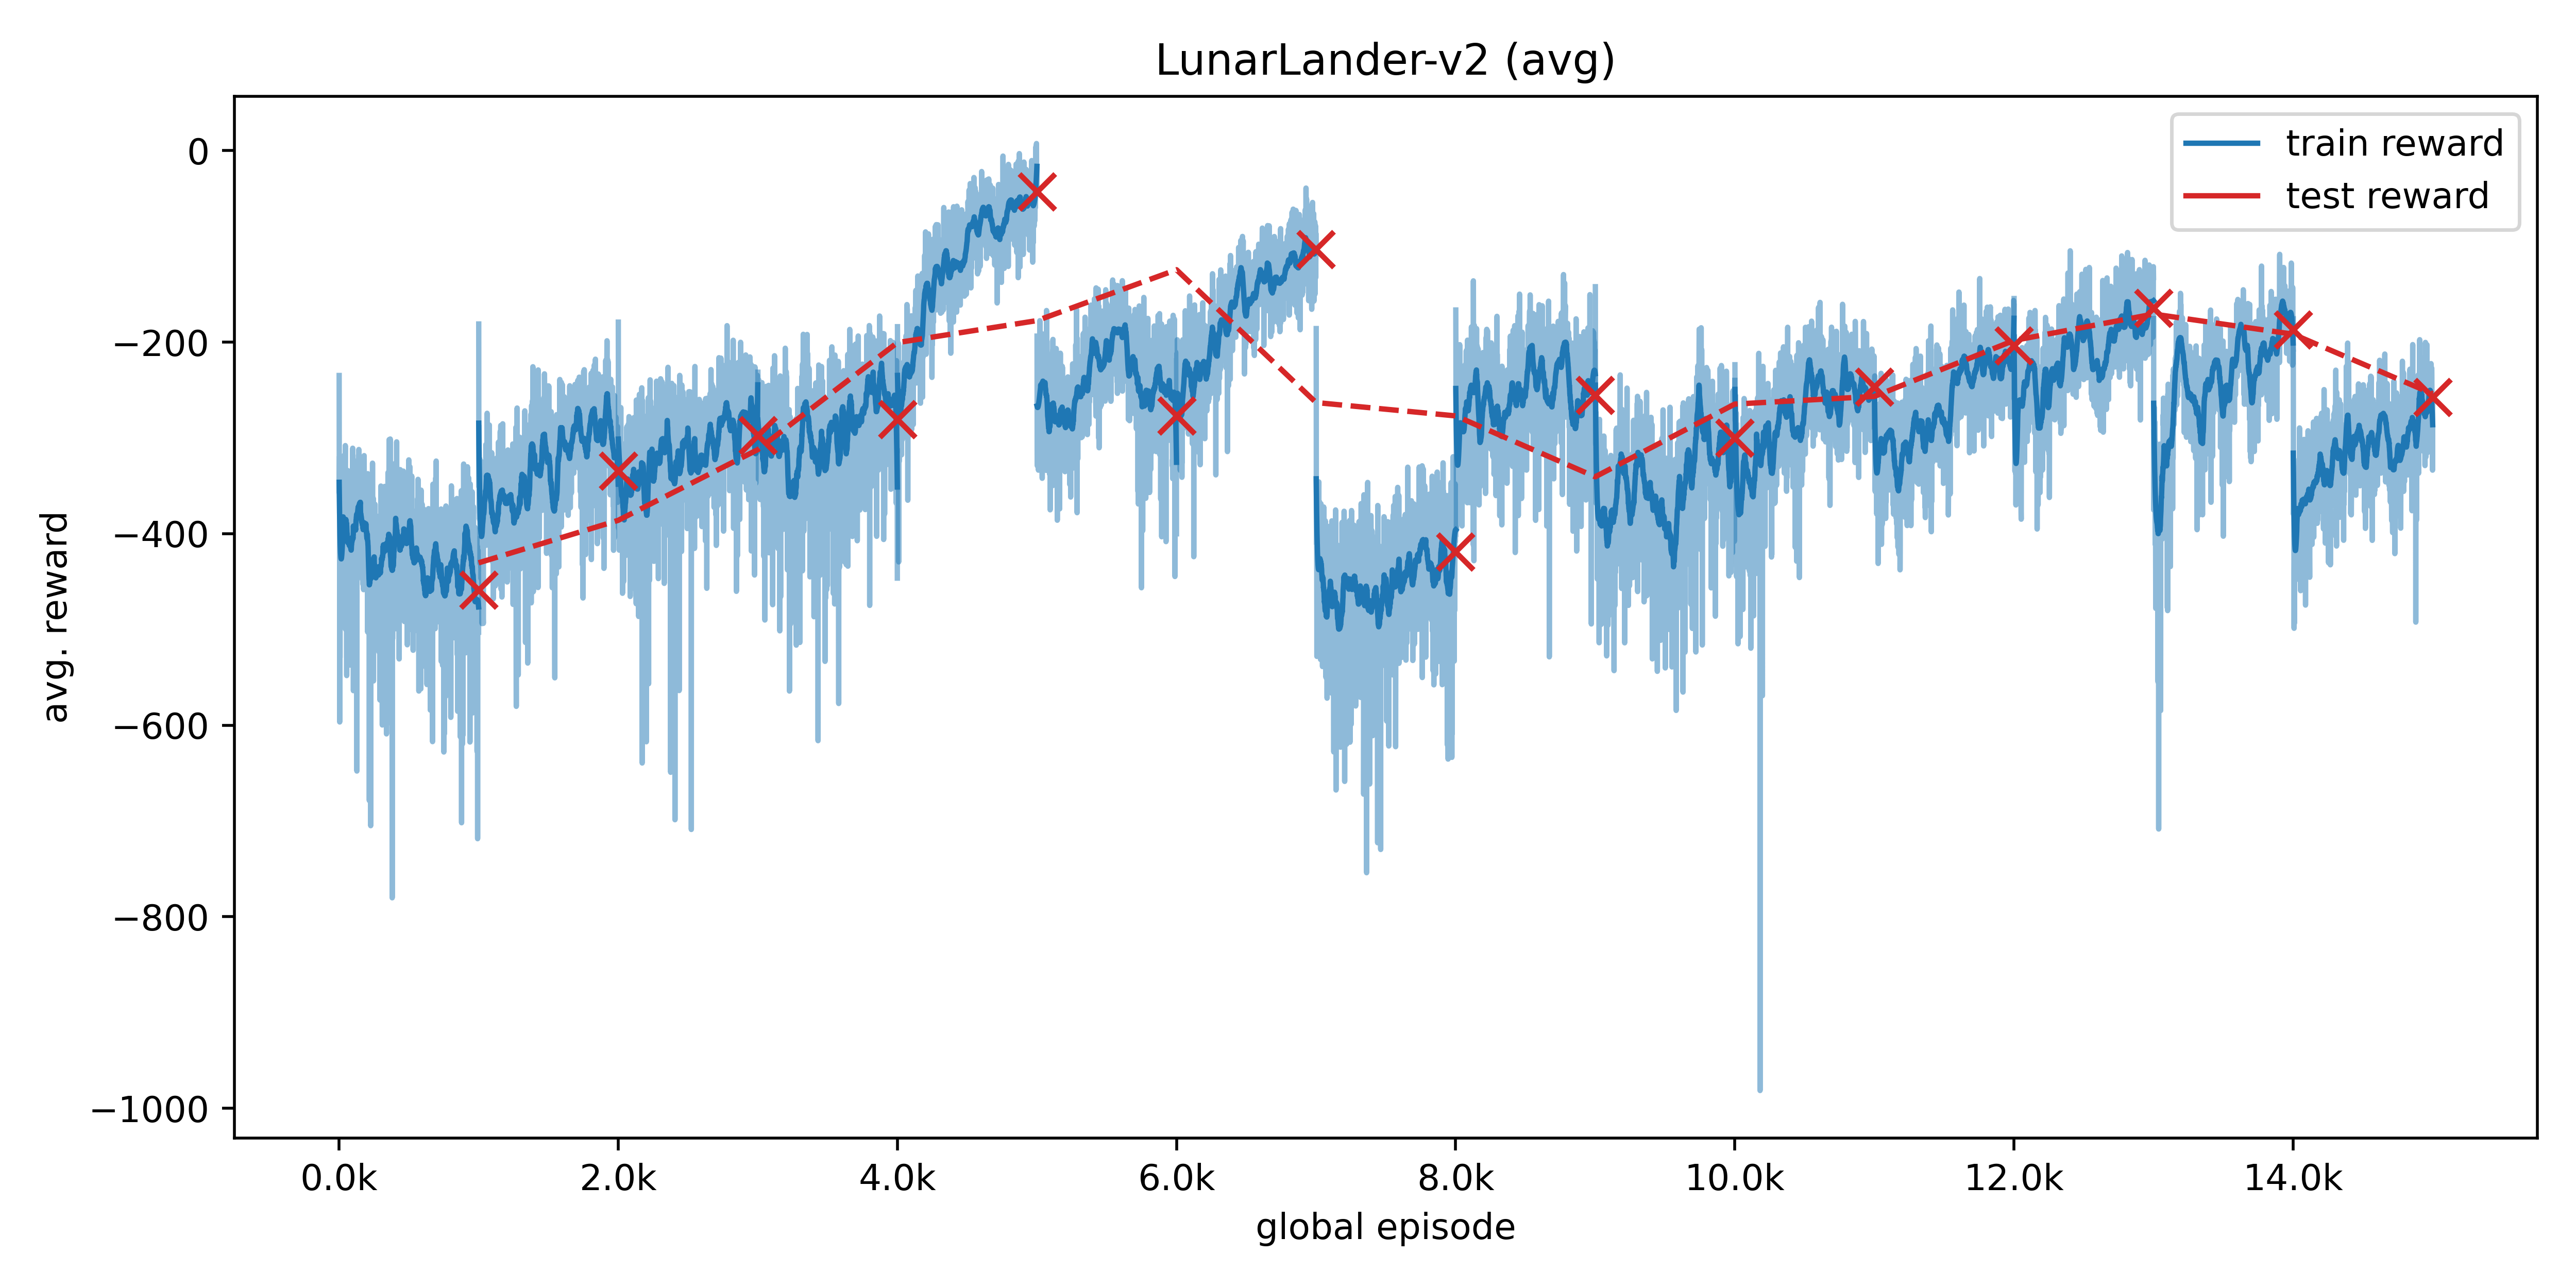
\includegraphics[width=0.9\linewidth]{figs/ll_avg_rewards.png}
    \caption{
        Average reward per global episode number for the LunarLander environment.
    }
    \label{fig:avg-ll}
\end{figure}

\begin{figure}[htbp]
    \centering
    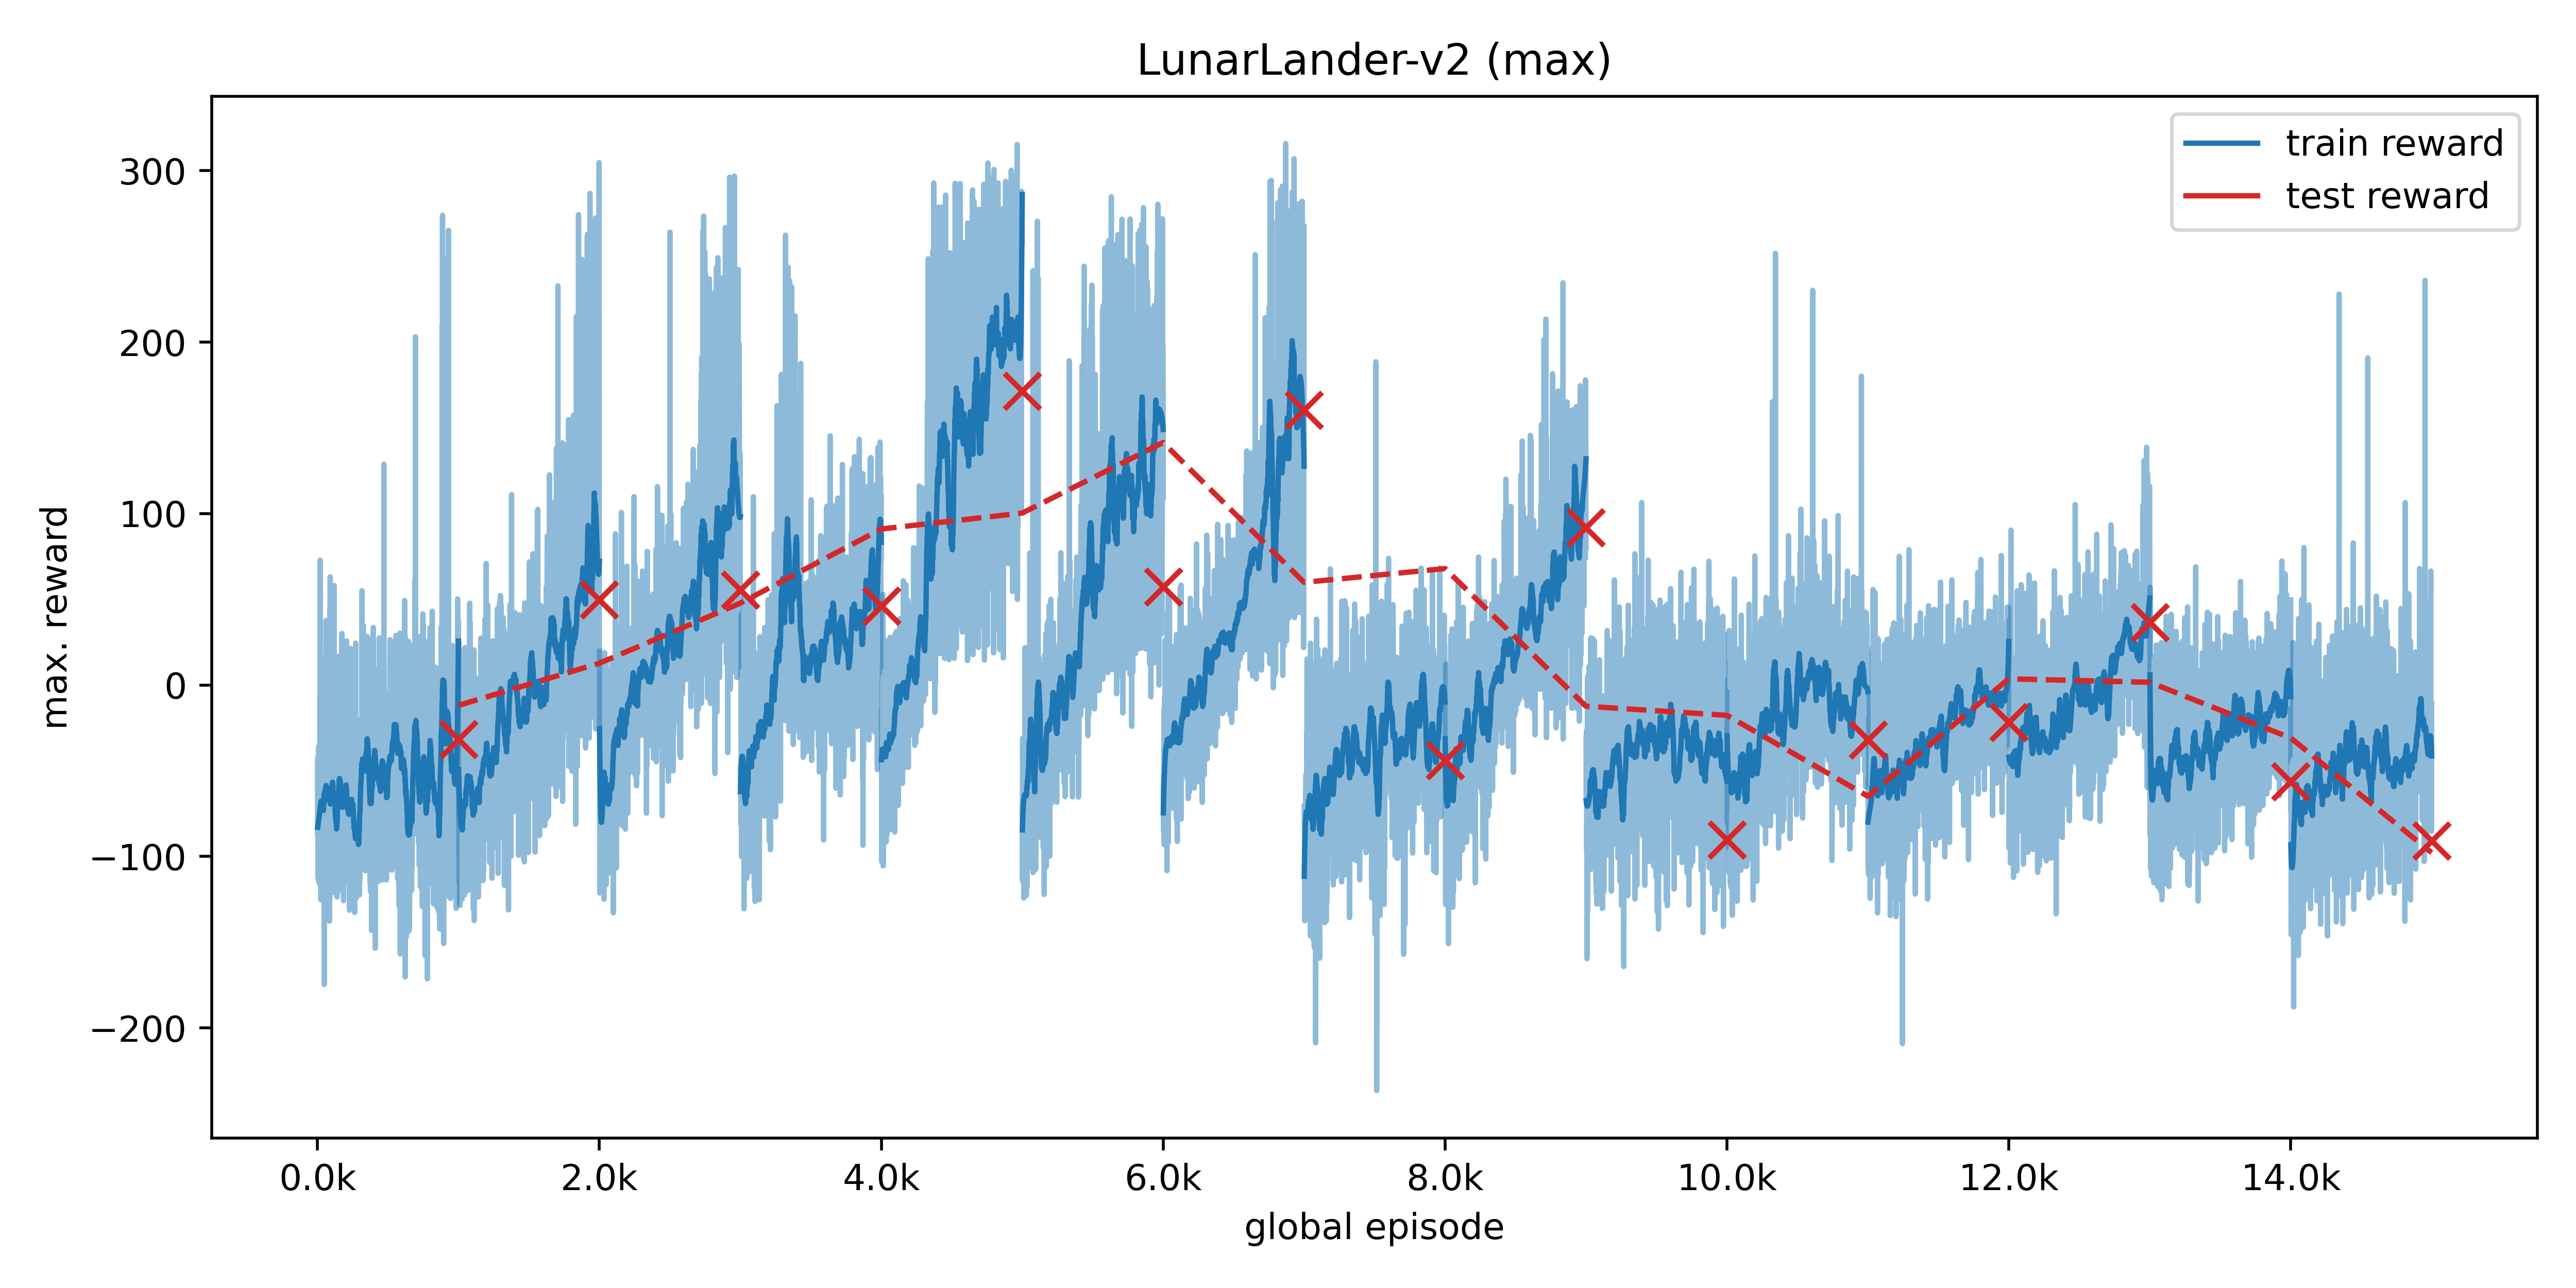
\includegraphics[width=0.9\linewidth]{figs/ll_max_rewards.png}
    \caption{
        Maximum reward per global episode number for the LunarLander environment.
    }
    \label{fig:max-ll}
\end{figure}

% -------------------------------------------------------------------
% -------------------------------------------------------------------
\section{Conclusion}
\label{sec:conc}

\TODO{
    What did we find, why are some architectures/params better than others for specific environment?
    Is EA a valid approach for this problem?
}

\section{Discussion}
\label{sec:disc}

While carrying out this research, we came across a number of ways it could be improved or expanded upon. In this section, we will discuss these topics. 

One of the main probelms we encountered during this project is amount of resources it takes to optimize the parameters. Each candidate configuration produced by the evolutionary algorithm needs to be fully trained on an environment, preferably multiple times to reduce variance. 
To be able to carry out the project some compromises had to be made to reduce the resource costs. 

The first place we made these compromises is the evolutionary algorithm, where we put a very strong emphasis on exploiting the population and sacrificed exploration. Exploration is important in optimization problems when the search space contains multiple local minima. 
With such strong focus on exploitation, the algorithm will converge on the local minimum closest to its initial conditions, without any guarantee that this is a good minimum. Exploration allows the algorithm to escape weak minima and converge onto stronger ones. 
Given our limited resources, finding any local minimum is considered a good proof of concept result. If this method were to be used in practice, it would be beneficial to change some parts of the EA to focus more on exploration.
For example, deterministic selection could be replaced with tournament selection, which selects each individual by randomly selecting a pool of candidates and adding the best one to the offspring pool. This allows for bad candidates to be filtered out without always choosing the absolute best ones. 

The resource cost was also reduced by severely limiting the search space for the A2C parameters. Each parameter was discretized to have two or four options, so that we could encode them in one or two bits for the EA. 
This means that the optimal value for each parameter will only be approximated. It also means that some interesting configurations will not be considered. For example, there is only a single parameter for the number of nodes in the hidden layers. Many modern architectures are not so simple and instead layers tend to increase or decrease in size as we proceed further into the network. 
When repeating this project with more resources there should be more options for the discrete variables and extra variables for neural architecture. In addition, an genetic algorithm capable of working with continuous variables such as Differential Evolution \cite{DifferentialEvolution} could be used.  


\TODO{
    What could be improved?
    What could be done differently?
    What could be done next?
}

% -------------------------------------------------------------------
\bibliography{references}

\end{document}
